\documentclass{article}

% Language setting
% Replace `english' with e.g. `spanish' to change the document language
\usepackage[english]{babel}

% Set page size and margins
% Replace `letterpaper' with`a4paper' for UK/EU standard size
\usepackage[letterpaper,top=2cm,bottom=2cm,left=3cm,right=3cm,marginparwidth=1.75cm]{geometry}

% Useful packages
\usepackage{amsmath}
\usepackage{graphicx}
\usepackage[colorlinks=true, allcolors=blue]{hyperref}

\usepackage{chronology}
\usepackage{url}
\usepackage{amsfonts}
\usepackage[most]{tcolorbox}
 	\definecolor{seashell}{rgb}{1.0, 0.96, 0.93}
	\definecolor{beaublue}{rgb}{0.74, 0.83, 0.9}
\tcbset{colback=seashell, colframe=beaublue, 
        highlight math style= {enhanced, %<-- needed for the ’remember’ options
            colframe=red,colback=red!10!white,boxsep=0pt}
	    }

\makeatletter
\renewcommand*\env@matrix[1][*\c@MaxMatrixCols c]{%
  \hskip -\arraycolsep
  \let\@ifnextchar\new@ifnextchar
  \array{#1}}
\makeatother

\usepackage{color}
\usepackage{tikz}
\usepackage{soul}
\usepackage{caption}
\usepackage{subcaption}
\usepackage{float}
\usepackage{mathtools}
	
\newcommand{\plain}{\color{black}}

\definecolor{c1}{RGB}{114,0,172}   % primary
\definecolor{c2}{RGB}{45,177,93}   % true
\definecolor{c3}{RGB}{251,0,29}    % false
\definecolor{c4}{RGB}{18,110,213}  % secondary
\definecolor{c5}{RGB}{255,160,109} % tertiary
\definecolor{c6}{RGB}{219,78,158}  % alt-primary

\newcommand{\growth}{\color{c1}}
\newcommand{\unitQuantity}{\color{c2}}
\newcommand{\unitInterest}{\color{c3}}
\newcommand{\unitTime}{\color{c4}}
\newcommand{\perfectly}{\color{c5}}
\newcommand{\compounded}{\color{c6}}
	

\title{\Large Seminar: Computational Methods for X-ray Computed Tomography \\
[5mm] \normalsize Session 1 \\
}
\author{Rayen Manai}
\date{April 19, 2023}
\begin{document}
\maketitle

\begin{abstract}
I present an Introduction to X-ray computed tomography and the basic mathematics needed for it. 
\newline 
	This work is based on the first three chapters of the book \href{https://epubs.siam.org/doi/book/10.1137/1.9781611976670}{Computed Tomography: Algorithms, Insight, and Just Enough Theory}~\cite{hansen2021computed} by Per Christian Hansen, Jakob Sauer Jorgensen, and William R.B. Lionheart. 
\newline 
	The code implemented to generate the visualizations in this work can be found in the following repository: \href{https://github.com/RayenManai/CT-Math-Visualizations.git}{https://github.com/RayenManai/CT-Math-Visualizations.git}
\end{abstract}

\tableofcontents
\pagebreak
\section{Introduction}
X-ray computed tomography commonly known as CT scanning is a non-invasive medical imaging technique that uses X-rays to produce detailed images of the internal structures of the body. The method involves rotating an X-ray source around the patient while taking multiple X-ray measurements from various angles. These measurements are then processed using complex mathematical algorithms to generate detailed 3D images of the body's internal structures.
In this work I will give an Introduction to X-ray computed tomography and the basic mathematics needed for it. 

 \subsection{What is Tomography?}
 The term "tomography" is derived from the Greek words $tomos$ meaning a section or slice, and $graphos$ meaning to describe. Tomography involves generating images of an object's slices without physically cutting it.
\newline
Typically this is done by measuring the transmission of waves or particles which more or less travel in straight lines but whose intensity is attenuated by the material through which they travel.
\newline
In most cases, the production of these images is based on the mathematical procedure tomographic reconstruction, which will be covered in detail through this course.
 \subsection{Important Applications of tomographic imaging}
 \begin{itemize}
	 \item \textbf{Medical and biological imaging: }
		 Clinical X-ray CT scanning is a common imaging modality used in medical settings to visualize bone and tooth damage, as well as soft tissues like the lungs. In laboratory settings, X-ray CT is used to image tissue samples on a smaller scale, while electron tomography is capable of imaging even smaller objects such as viruses with high resolution.
	 \item \textbf{Non destructive inspection and testing: }
In manufacturing, X-ray CT is used to identify defects in products and verify dimensional accuracy. X-ray and gamma ray tomography are employed to monitor the content and integrity of oil and gas pipes. 
		 In museums, tomography enables non-invasive investigation of artistic and cultural artifacts, archaeological finds, and fossils, without causing damage.
	 \item \textbf{Materials science: }
		 For the development of advanced materials with superior properties, it is essential to gain a comprehensive understanding of their micro- and nano-scale characteristics. A range of imaging techniques is employed to study and develop materials, including laboratory X-ray tomography, high-energy synchrotron X-ray tomography, neutron tomography, and transmission electron microscopy (TEM) tomography.
	 \item \textbf{Security Screening: }
		 X-ray CT technology finds extensive use in the inspection of parcels and luggage, especially at airports. By providing a 3D view, it allows for the detection of objects that might otherwise remain hidden beneath denser items. Along with its application in detecting bombs and weapons, tomography is also employed to detect contraband.

 \end{itemize}
 \subsection{CT between the past and the present}
 \subsubsection{Some history}
\begin{chronology}[15]{1895}{2000}{110ex}[\textwidth]
	\event {1895}{X-ray Discovery}
	\event{1917} {Johann Radon}
	\event [1956]{1964}{2 Important Papers}
	\event [1971]{1972}{First Application}
	\event {1979}{Nobel Prize}
\end{chronology}
\begin{itemize}
	\item In 1895, Wilhelm Conrad Röntgen discovered X-rays, which established the fundamental principles of X-ray scanners and tomography in the field of physics.
\item The mathematical aspect of this story can be traced back to 1917, when Johann Radon published a paper that dealt with the abstract problem of reconstructing a function on a plane from its line integrals.
\item The earliest known proposed use of tomography was in radio astronomy, which was outlined in Bracewell's paper in 1956. However, the actual beginnings of tomography are often attributed to Allan Cormack's 1963 paper, which was published in the 1960s.
\newline 
In 1964, Cormack conducted experimental measurements and documented his findings. Meanwhile, Godfrey Hounsfield had also developed an experimental X-ray tomography system. He first used it on a preserved human brain and later on animal brains obtained from butcher shops.
\item The system was first tested on a patient in 1971, and a patent was
granted in 1972
\item Hounsfield and Cormack jointly won the Nobel Prize in Physiology or
Medicine in 1979 for the invention of X-ray CT.
	
\end{itemize}
 \subsubsection{Tomography today}
 \begin{itemize}
	 \item \textbf{Cone-beam CT}
		 \newline
		 The majority of modern medical CT machines use a helical-scan cone beam in which the patient is translated on a table while the X-ray source and the detector array rotate about a horizontal axis, so the source describes a helix relative to the patient.
		 \newline
\vspace{0.2cm}
\newline
\fbox{%
\begin{minipage}{0.4\textwidth}
  \centering
  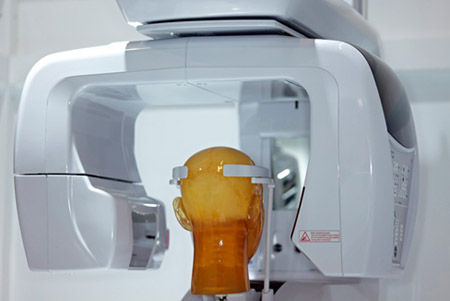
\includegraphics[scale = 0.3]{media/dental_cone_beam.jpg}
	\captionof{figure}{Dental cone-beam CT ~\cite{cone_beam_ct}}
\end{minipage}
\hfill
\begin{minipage}{0.6\textwidth}
	Dental cone-beam CT is widely used, not for everyday dentistry but in dental hospitals, often for patients undergoing extensive surgical procedures. These machines use a circular-scan cone-beam geometry.
\end{minipage}
}


	 \item \textbf{Positron Emission Tomography}
 \newline
		 We mention also emission CT methods e.g., positron emission tomography (PET) measures pairs of positrons given off by a nuclear reaction.		 \newline	
		 \vspace{0.2cm}
\newline
\fbox{%
\begin{minipage}{0.4\textwidth}
  \centering
  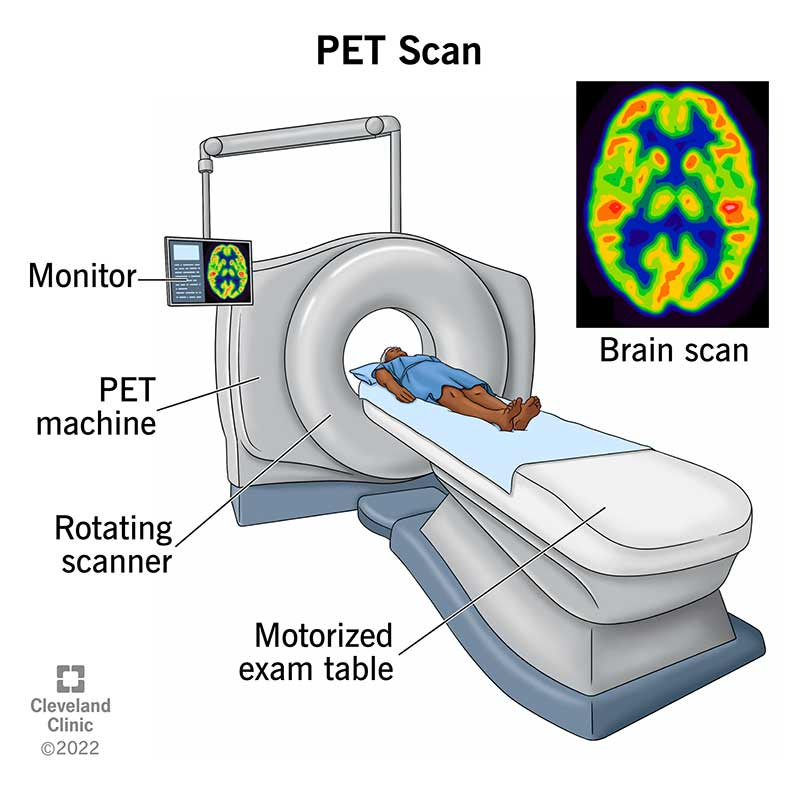
\includegraphics[scale = 0.2]{media/pet-scan.jpg}
	\captionof{figure}{Positron Emission Tompgraphy Scan ~\cite{pet_scan}}
\end{minipage}
\hfill
\begin{minipage}{0.6\textwidth}
	PET scans use a radioactive tracer to show how an organ is functioning in real time.  
	They can measure vital functions, such as blood flow, oxygen use and blood sugar (glucose) metabolism.~\cite{pet_scan}
They can also be combined with CT or MRI to image both metabolism and anatomy.
\end{minipage}
}

	 \item \textbf{Transmission Electron Microscope}
 \newline
		 Tomographic reconstruction is also widely used in transmission electron microscopy (TEM), particularly in a technique called cryo-EM, which is extensively applied in biology and medicine. In cryo-EM, the sample is frozen, and the charged nature of electrons allows them to be directed using magnetic and electric fields.
\newline
		 \vspace{0.2cm}
\newline
\fbox{%
\begin{minipage}{0.4\textwidth}
  \centering
  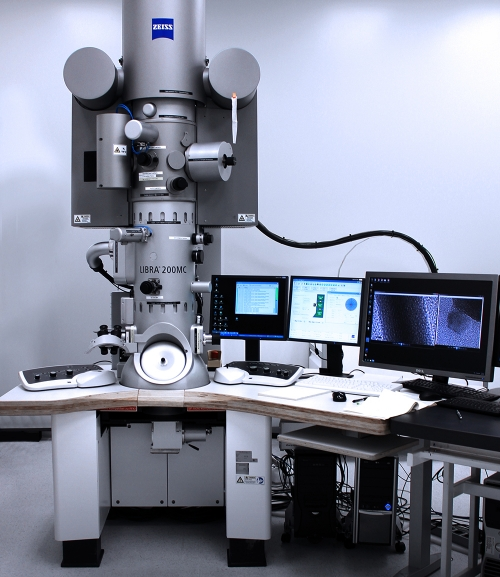
\includegraphics[scale = 0.2]{media/tem.jpg}
	\captionof{figure}{Transmission Electron Microscope ~\cite{tem}}
\end{minipage}
\hfill
\begin{minipage}{0.6\textwidth}
	Commonly this uses a scanning transmission electron microscope (STEM), where a pencil beam of high-energy
electrons is focused into a narrow beam which is raster scanned, or an ordinary TEM, in which the full object is illuminated by a parallel beam.
\end{minipage}
}
\newline
\vspace{0.2cm}
\newline
This technique is used, e.g., to image virus particles. The Electron Microscopy Data Bank reported that 200 out of the 250 protein structures registered in 2020 were found using electron tomography.
	 \item \textbf{Synchrotron X-ray Source}
 \newline
X-ray tomography at a higher resolution than possible on a laboratory system can be performed using a synchrotron X-ray source. This can be a high-intensity beam that is highly collimated and close to monochromatic.
		 \newline 
		 \vspace{0.2cm}
\newline
\fbox{%
\begin{minipage}{0.4\textwidth}
  \centering
  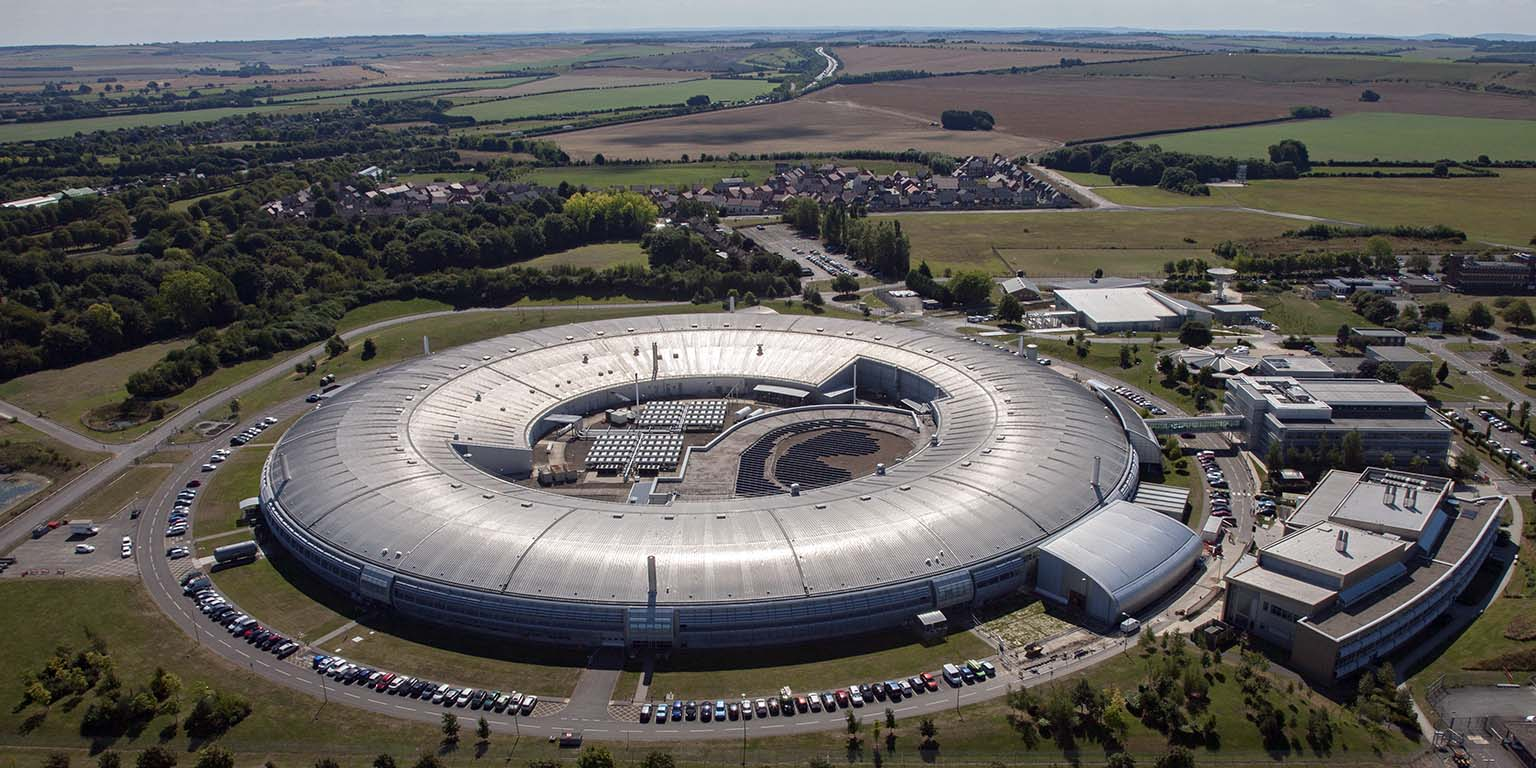
\includegraphics[scale = 0.11]{media/synchrotron.jpg}
	\captionof{figure}{Diamond Light Source: the UK’s national synchrotron ~\cite{synchrotron}}
\end{minipage}
\hfill
\begin{minipage}{0.6\textwidth}
	Synchrotron X-ray sources are usually found at large national or multinational facilities, such as the Diamond Light Source located in Harwell, UK, or the European Synchrotron Radiation Facility (ESRF) in Grenoble, France. Due to the high cost of these facilities, there is often a concentrated effort to achieve the best possible reconstruction results.

\end{minipage}
}

 \end{itemize}
\subsection{Aim and contents of the book}

\begin{itemize}
	 \item chapters 2, 3: we review necessary mathematical theory and concepts
	 \item chapter 4: this outlines the physics of X-ray tomography
	 \item chapter 5: we introduce the forwrad operator, the Radon transform that takes the image to the data.
	 \item chapter 6: we discuss the most common family of analytical inversion methods, Filtered Back Projection.
	 \item chapter 7: limited-data problems: singular values and functions of the Radon transform.
\item chapter 8: this employs tools from microlocal analysis to look carefully at what can and cannot be stably retrieved from such restricted data.
\item chapter 9: this covers the process of going from a continuum problem to a discrete one
\item chapter 10: this marks a transition from problems in functional analysis to a focus on numerical linear algebra and optimization.
\item chapter 11: this introduces the numerical linear algebra approach to image reconstruction in tomography
\item chapter 12: this examines inverse problems and regularization; a trade-off between fitting the data and imposing prior assumptions about the image.
\item chapter 13: we cover modern practical optimization methods that can be applied to tomographic imaging
\end{itemize}
\section{Analysis Background}
\subsection{Linear Operators}
We are intersted in the study of operators because most of the problems in tomography will be formulated as an operator that takes an image to some data.
\newline
An operator is a function that takes a function and gives another function.
\newline
\vspace{0.1cm}
\newline
\textbf{Notation: }for an operator $K$, we denote by $K[f]$ the function $f$ it is taken to and by $K[f](x)$ its value at a real number $x$.
\newline
\vspace{0,1cm}
\newline
\textbf{The range} is the set of all functions $K[f]$ for some valid $f$, and it is often a smaller set than the co-domain.
\vspace{0.5cm}
\newline
\textbf{example 1: Integration}
\newline
For a function $f$ : $[-\pi, \pi] \rightarrow [-\pi,\pi]$, we can regard the operation:
$$ K[f](y) \; \; = \; \; \int_{-\pi}^{y} f(x) \,dx$$
	as an operator whose domain and co-domain are integrable functions on the interval $[-\pi, \pi] $ 
	\newline 
	Integrating a function makes it a little smoother, so in this example the range is a smaller set than the co-domain.
\newline
\vspace{0.2cm}
\newline
\textbf{Linearity of an Operator:}
\newline
We say an operator is linear if it has both \textbf{the superposition property} 
	$$  K[f1 + f2] \; = \; K[f1] + K[f2]$$ 
	for any two functions f1 and f2 in the domain and \textbf{the scaling property} 
	$$ K[\alpha f] \; = \; \alpha K[f]$$
	for any function f in the domain and any scalar $\alpha$ .


\subsection{Convolution}
%% source : https://betterexplained.com/articles/intuitive-convolution/
	$$
	\plain ( 
	\growth f
\perfectly *
\unitTime g
	\plain )
	\plain (
	\unitInterest t
	\plain )
\plain =
	\unitQuantity \int_{-\infty}^{\infty} \growth f(\tau)
	\unitTime g(\unitInterest t \compounded -\tau \unitTime) \unitQuantity d\tau $$
\perfectly To convolve
\growth       a kernel
\plain        with an 
\unitTime input signal :
\
\compounded flip the signal
\unitInterest move to the desired time 
\unitQuantity and accumulate every interaction  
\growth with the kernel ~\cite{colorized}
\plain 
\vspace{0.5cm}
\newline
\textbf{example 2: Convolution operator for periodic functions} 
\newline
We consider again $2\pi$-periodic functions on the interval $[-\pi, \pi]$, and we define the convolution operator as: 
$$ g(x)  =  K[f](x)  = \int_{-\pi}^{\pi} h(y - x )f(y) \, dy $$  or $$ g  =  h * f$$
\begin{itemize}
		\item $h$ defines the system (periodic) 
		\item $y-x$ wraps around when it goes outside the interval $[-\pi, \pi]$
		\item we refer to convolution of periodic functions as \textbf{circular convolution}.
	\end{itemize}

\subsection{Inverse Problems and Regularization}
We will now discuss the inverse process of computing or reconstructing the function f from the data g, which we refer to as an inverse problem.
\subsubsection{What is an inverse problem?}

\begin{center}
\begin{tikzpicture}
	\node (pic1) at (0,0) {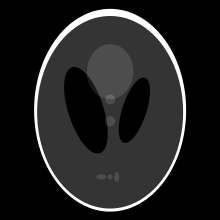
\includegraphics[width=0.15\textwidth]{media/SheppLogan_Phantom.png}};
\node (pic2) at (7,0) {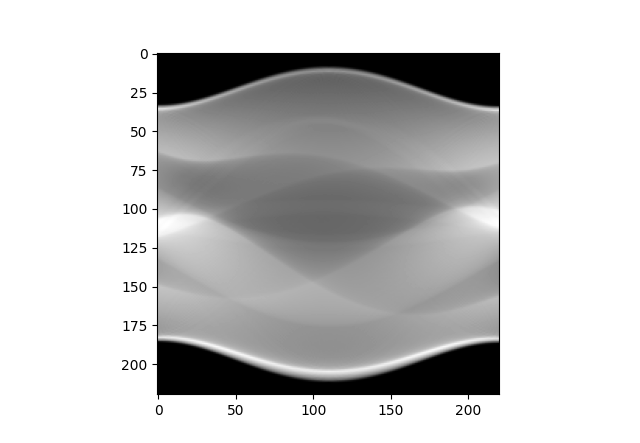
\includegraphics[width=0.25\textwidth]{media/sinogram.png}};
\draw[->,thick] (pic1.east) -- ++(2.2,0) |- (pic2.west) node[pos=0.5,above] {Direct Problem};
\draw[->,thick] (pic2.west) -- ++(-2.2,0) |- (pic1.east) node[pos=0.5,below] {Inverse Problem};
\end{tikzpicture}
\newline
Direct problem: given object $f$ determime data $y$
\newline
Inverse problem: given noisy data $ \hat{y}$, recover object $f$
\end{center}
In an inverse problem, the goal is to estimate a quantity $f$ that cannot be directly observed using indirect measurements $g$ and the forward model, represented by the operator $K$. The forward problem describes how the observations are generated, while the inverse problem is concerned with determining the causal factors that produced the observations based on the available data.
\newline
In an inverse problem, we usually start with a forward problem, such as "given the properties of the interior of the object, how much of an X-ray beam penetrates the object," and try to invert it by deducing information about the interior of the object from measurements obtained from the exterior.
\newline
The forward problem is usually governed by natural laws and solved by physics. However, as humans, we choose an inverse problem to solve, which is why these problems are often very challenging.
\newline
\begin{tcolorbox}[colback=seashell,colframe=beaublue,title= The Three Important Questions of Inverse Problems]
\begin{enumerate}
	\item \textbf{What do you need to find?} In many cases, the primary objective of imaging is not to generate high-quality images, but rather to address specific tasks such as detection, localization, quantification, or diagnosis. While obtaining a high-quality image may not always be feasible, it may still be possible to extract relevant information and answer more targeted questions. 
	\item \textbf{What can you measure?} For more reliable measurements, it is necessary to develop a robust model that accounts for various factors, such as measurement uncertainty and the distribution of measurement errors.
	\item \textbf{What do you already know?} Inverse problems tend to be ill-posed. Therefore prior knowledge plays a critical role in achieving stable image reconstruction. This prior knowledge may stem from a variety of sources, including known material properties of the sample. By leveraging such a priori information, it becomes possible to mitigate the ill-posed nature of inverse problems and achieve more accurate and reliable image reconstructions.

\end{enumerate}
\end{tcolorbox}
\subsubsection{Sensitivity to noise}
CT images can be affected by noise, which can result in reduced image quality and potentially lead to diagnostic errors.
\newline 
The noise can arise from various sources, such as electronic noise in the CT detector, scattered radiation, or patient motion during the scan and can lead to
artifacts in the reconstructed image, such as streaks or blurring.
\newline
That's why it is necessary to minimize the noise in CT scans to improve the image quality and the diagnostic accuracy.		 
\newline 
There are several mathematical methods to reduce noise in images, including:
\newline
\textbf{Filtering:} it is a technique that involves modifying pixel values in an image to reduce noise while preserving image details. There are various types of filters that can be used, such as mean, median, Gaussian, and Wiener filters with which we can avoid most of the noise at the cost of
losing some details.

\begin{figure}[H]
  \centering
\fbox{%
\begin{minipage}{\textwidth}
	\begin{center}
  \begin{subfigure}[b]{0.6\textwidth}
  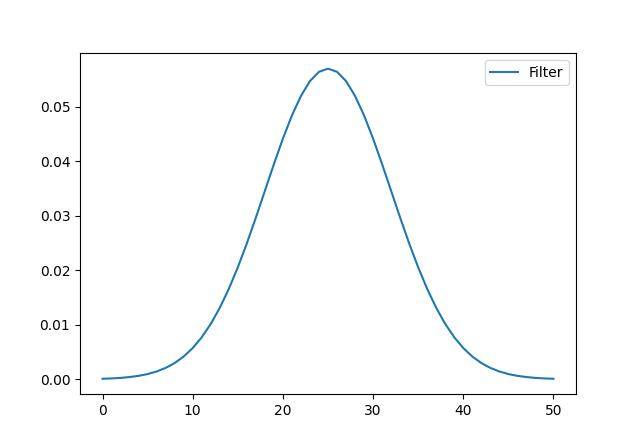
\includegraphics[scale = 0.5]{media/gaussian.png}
    \caption{Filter}
    \label{fig:f1}
  \end{subfigure}
  \begin{subfigure}[b]{0.9\textwidth}
	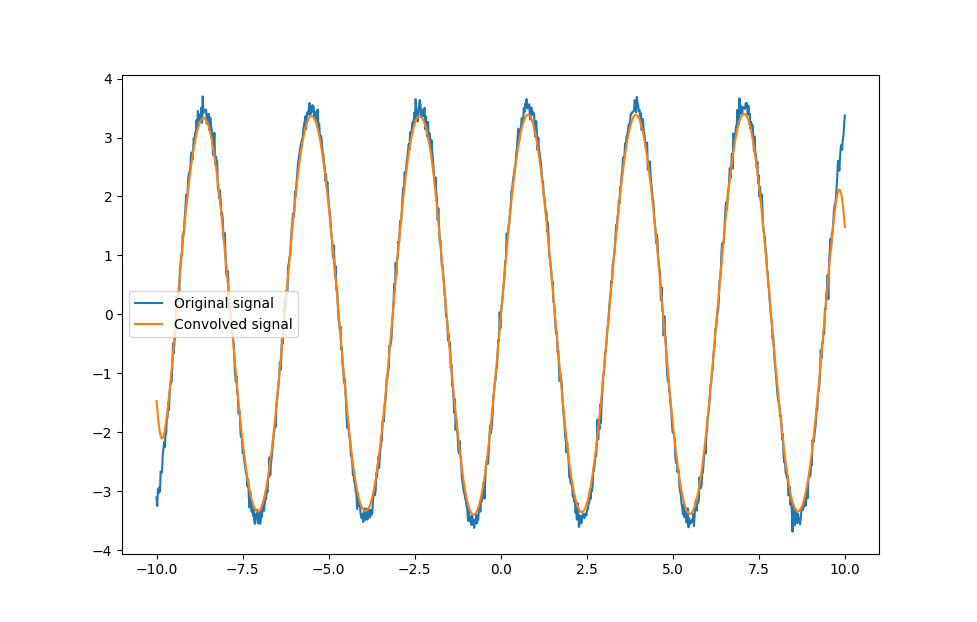
\includegraphics[scale = 0.5]{media/noise_mixed.png}
    \caption{result}
    \label{fig:f2}
  \end{subfigure}
\end{center}
\end{minipage}
	}
	\caption{Applying a filter to a noisy signal}
  \label{fig:label}
\end{figure}


\subsubsection{Well posed and Ill posed problems}
Inverse problems can be quite difficult to solve. This is because many inverse problems are ill posed, according to the following definition:

\begin{tcolorbox}[colback=seashell,colframe=beaublue,title= Hadamard’s criteria for a well-posed problem]
	\begin{itemize}
		\item a solution exists
		\item the solution is unique
		\item the solution depends stably on the data
	\end{itemize}
		If a problem violates any of these criteria, we say that it is ill posed.
\end{tcolorbox}
\textbf{Stability:}
\newline
The solution is stable if any perturbation of the data $g$ produces a bounded perturbation of the solution $f$.
\newline
On the other hand, by instability we mean that a small perturbation in the data can make an arbitrarily large change in the solution $f$.
\subsubsection{Stabilization by Regularization}
Suppose the operator $K : U \rightarrow V  $ has a bounded inverse but, the noisy data $g$ lives in a co-domain larger than the range, this means that there is no $f$ such that $ K[f] = g$ and the first Hadamard criterion is violated. 	 
 \newline	
		 \vspace{0.1cm}
\newline
	To overcome this, it is common to instead consider a solution that minimizes a norm of the residual $K[f] - g$: 
	$$ f_{min} = argmin_{f} || K[f] - g ||_{V}^{2} $$	  
	\vspace{0.1cm}
         \newline
	\textbf{Regularization:} a class of solution methods designed to make the solution regular, stable with respect to perturbations. This can be achieved through: 
	\begin{itemize}
		\item altering the reconstruction so the modified problem satisfies the three Hadamard criteria, generally known as Tikhonov regularization (more in the discrete setting in chapter 12)
		\item regularizing the solution by introducing filters in the expansion (filtering techniques in Chapters 6, 7, 10, 11 and 12)
		\item terminating an iterative solver before the noise starts to dominate the reconstruction (this approach is discussed in Chapter 11)
	\end{itemize}
\subsection{The Fourier Transform}
There are various conventions in defining the Fourier transform. Here, we define \textbf{the Fourier Transform} for a function $f$ of one variable $x$ by: 
\begin{equation}
	\tcboxmath {\hat{f(\omega)} = \frac{1}{\sqrt{2\pi}} \int_{-\infty}^{\infty}f(x)e^{-ix\omega} \, dx}
\end{equation}
where the Fourier-transformed function $f$ is a function of the angular frequency $\omega$. 
\newline
\vspace{0,1cm}
\newline
\textbf{The inverse Fourier Transform} of a function f is then defined as: 
\begin{equation}
	\tcboxmath {\check{f(x)} = \frac{1}{\sqrt{2\pi}} \int_{-\infty}^{\infty}f(\omega)e^{ix\omega} \, d\omega}
\end{equation}
Examples:
\begin{figure}[H]
  \centering
\fbox{%
\begin{minipage}{0.5\textwidth}
  \centering
  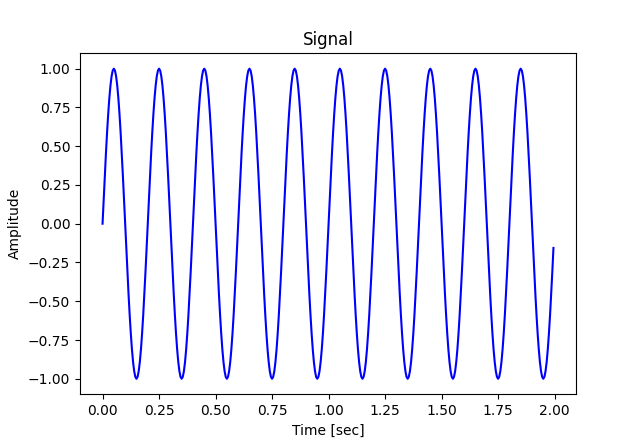
\includegraphics[scale = 0.5]{media/signal2.png}
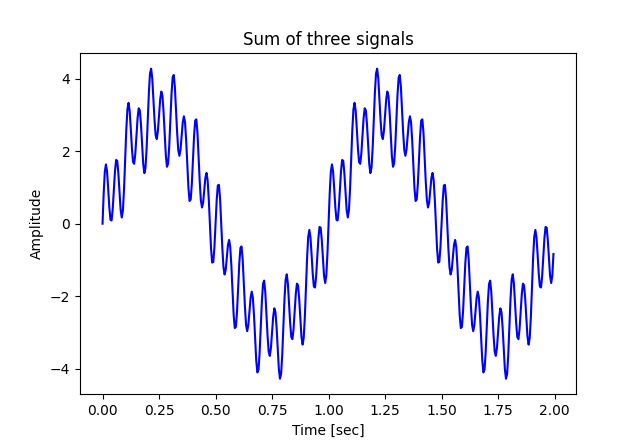
\includegraphics[scale = 0.5]{media/signal3.png}

\end{minipage}
\hfill
\begin{minipage}{0.5\textwidth}
	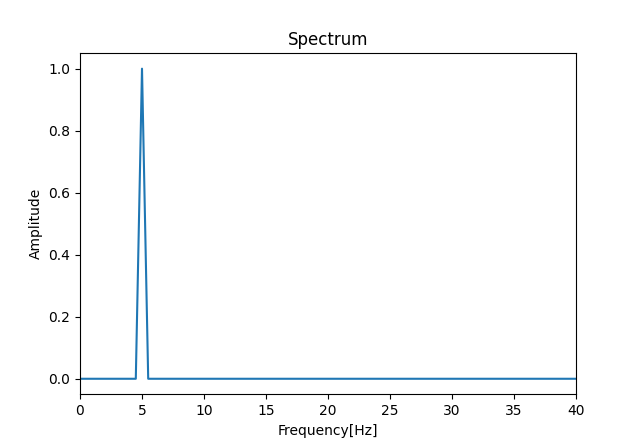
\includegraphics[scale = 0.5]{media/fourier2.png}
	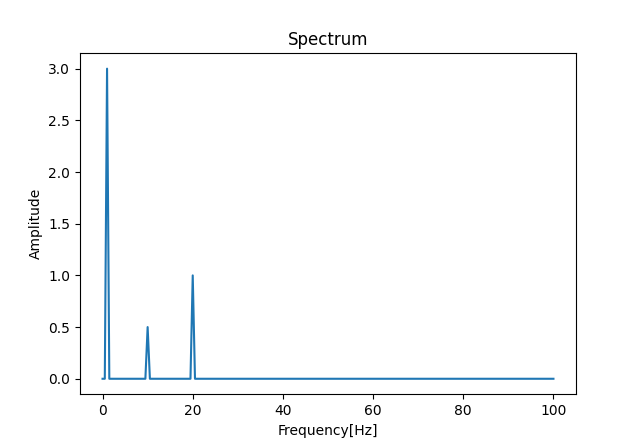
\includegraphics[scale = 0.5]{media/fourier3.png}
\end{minipage}
	}
  \caption{Signals and their corresponding Fourier Transform Spectrums: A visualization of the frequency content of a signal obtained through Fourier Transform.
	\newline 
	The left side shows the signal in the spatial domain, while the right side displays its corresponding frequency domain representation.}
  \label{fig:label}
\end{figure}
\textbf{The 2D Fourier Transform: }
	Let $f$ be a function of $x = (x_1,x_2)$. The the 2D Fourier Transform is a function of the angular frequency vector $\omega = (\omega_{1},\omega_{2})$ given by :
	\begin{equation}	
		\tcboxmath{\hat{f(\omega)} = \frac{1}{2\pi}\int_{-\infty}^{\infty} \int_{-\infty}^{\infty}f(x)e^{-ix\omega} \, dx_{1}dx_{2}}
	\end{equation}

	where $ x\omega = x_1\omega_{1} + x_2 \omega_{2}$
\newline 
\vspace{0.1cm}
\newline
\textbf{The 2D inverse Fourier Transform: }
\begin{equation}
		\tcboxmath {\check{f(x)} = \frac{1}{2\pi}\int_{-\infty}^{\infty} \int_{-\infty}^{\infty}f(\omega)e^{ix\omega} \, d\omega_{1} d\omega_{2}}
\end{equation}
	$\rightarrow$ The 2D Fourier Transform is just the 1D Fourier Transform with respect to each of the variables in turn.

\subsection{Convolution using the Fourier Transform}

\textbf{The convolution theorem: }this states that the Fourier Transform of the convolution of two functions is equal to the product of their Fourier transforms.
\newline
This means that finding the convolution of two functions in spatial domain is equivalent to multiplying the Fourier transforms of the two functions in frequency domain.

\begin{center}
\begin{tabular}{|c|c|}
\hline
\textbf{Spatial Domain} & \textbf{Frequency Domain} \\
\hline
	$g(x) = f(x)*h(x) $& $G(\omega) = F(\omega)H(\omega)$ \\
	$\downarrow$ & $\downarrow$ \\
	Convolution & Multiplication \\ 
\hline
\end{tabular}
\end{center}
\fbox{%
\begin{minipage}{0.4\textwidth}
  \centering
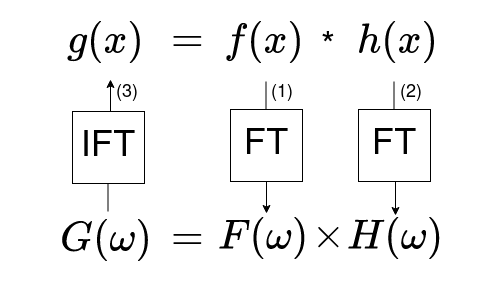
\includegraphics [scale=0.3]{media/convolution&fourier.png}
\end{minipage}
\hfill
\begin{minipage}{0.6\textwidth}
	To compute $g(x) = f(x) * h(x)$, there is no need to perform the computation in the spatial domain. Instead one can (1) take the Fourier Transform of $f$ to get $F(\omega)$, (2) the Fourier Transform of $h$ to get $H(\omega)$, multiply the two, and then take (3) the inverse Fourier Transform of $G(\omega)$ to get $g(x)$.
\newline
This approach is computationally efficient as there exist fast algorithms for finding the Fourier transform and inverse Fourier transform. Additionally, this method enables the examination of the impact of filter application by evaluating the effects of spatial filters in the frequency domain and vice versa.
\end{minipage}
}
\section{Linear Algebra Background}
\subsection{System of Linear Equations}
When we discretize a CT reconstruction problem, we arrive at a system of linear equations $Ax = b$, where the matrix $A$ represents a linear operator, $b$ is the right-hand side vector holding the measured data, and the vector $x$ is the unknown solution which represents the reconstruction we want to compute.
\subsubsection{Notation}
	column vector: $ v = \begin{pmatrix} v_1 \\ \vdots \\ v_n \end{pmatrix} \;$ , 
	row vector: $v^\top = \begin{pmatrix} v_1 & v_2 & \cdots & v_n \end{pmatrix} $
		\newline 
		If the matrix $A$ has dimensions $ m \times n $ (m rows and n columns), then we write it as : 
\[
A = \begin{pmatrix}
    \vert & \vert & \dots & \vert \\
    \mathbf{c_1} & \mathbf{c_2} & \dots & \mathbf{c_n} \\
    \vert & \vert & \dots & \vert
\end{pmatrix}
\quad=
\begin{pmatrix}
    \text{\textbf{r}}_1 \\
    \text{\textbf{r}}_2 \\
    \vdots \\
    \text{\textbf{r}}_m
\end{pmatrix}
\]
\subsection{Rank, Range and Null Space}
\begin{tcolorbox}[colback=seashell,colframe=beaublue,title=Rank]	
	The rank $r$ of an $ m \times n $  matrix $A$ is the number of linearly independent rows of
the matrix (it is also equal to the number of linearly independent columns), and
			 for a nonzero matrix the rank satisfies $ 1 \leq r \leq min(m,n) $
\end{tcolorbox}
			
			 \textbf{Example: } 
	 $$
		 \begin{pmatrix} 1 & 2 & 3 \\ 4 & 5 & 6 \\ 7 & 8 & 9 \end{pmatrix}  
			 \xrightarrow{r_2 - 4 \times r_1 \, \& \, r_3 - 7 \times r_1}
\begin{pmatrix} 1 & 2 & 3 \\ 0 & -3 & -6 \\ 0 & -6 & -12 \end{pmatrix}  
				\xrightarrow{r_3 - 2 \times r_2}
\begin{pmatrix} 1 & 2 & 3 \\ 0 & -3 & -6 \\ 0 & 0 & 0 \end{pmatrix}  
				 $$
				 
				 So this matrix has the rank $r = 2$

\begin{tcolorbox}[colback=seashell,colframe=beaublue,title=Range]	
The range, or column space, Range($A$), of an $m \times n$ matrix $A$ is the linear
subspace spanned by the columns of the matrix:
			 $$ Range(A) \equiv \{u \in \mathbb{R}^{m} | u = \alpha_1 c_1 + \alpha_2 c_2 + \hdots + \alpha_n c_n , arbitrary \; \alpha_j \} $$
		 
\end{tcolorbox}
 \textbf{Example: } 
		 $$
			A = \begin{pmatrix} 1 & 1 & 1 \\ 1 & 2 & 4 \\ 2 & 3 & 5 \end{pmatrix} \; 
				\xrightarrow{c_3 - c_1 \, \& \, c_2 - c_1}
			 \begin{pmatrix} 1 & 0 & 0 \\ 1 & 1 & 3 \\ 2 & 1 & 3 \end{pmatrix} \; 
				 \xrightarrow{c_3 - 3\times c_2}
	         \begin{pmatrix} 1 & 0 & 0 \\ 1 & 1 & 0 \\ 2 & 1 & 0 \end{pmatrix} \; $$		
				 So this Matrix has Rank = 2 and $ Range (A) = \alpha_1 \begin{pmatrix} 1\\ 1 \\ 2 \end{pmatrix} \; +   \alpha_2 \begin{pmatrix} 0\\ 1 \\ 1 \end{pmatrix} \; $
\begin{tcolorbox}[colback=seashell,colframe=beaublue,title=Null Space]	

The null space (or kernel), Null($A$), is the linear subspace of all vectors mapped to zero:
			 $$ Null(A) \equiv \{v \in \mathbb{R}^{n} | Av = 0 \} $$
\end{tcolorbox}
		  \textbf{Example:} 
			 $$
			A =  \begin{pmatrix} 1 & 1 & 1 \\ 1 & 2 & 4 \\ 2 & 3 & 5 \end{pmatrix} \; 
				\xrightarrow{r_2 - r_1 \, \& \, r_3-2\times r_1}
			 \begin{pmatrix} 1 & 1 & 1 \\ 0 & 1 & 3 \\ 0 & 1 & 3 \end{pmatrix} \; 
				 \xrightarrow{r_3 - r_2}
		         \begin{pmatrix} 1 & 1 & 1 \\ 0 & 1 & 3 \\ 0 & 0 & 0 \end{pmatrix} \; $$
				 So this Matrix has Rank = 2 and $ Null(A) = \alpha_1 \begin{pmatrix} 2\\ -3 \\ 1 \end{pmatrix} \; $

					 \subsection{Linear Least Squares Problem}
				The linear least-squares problem is probably the most well known problem formulation that seeks to handle inconsistency of a linear problem, i.e., to define a meaningful “solution” to an inconsistent system. 
				\newline 
				The key idea is to find an $x$ such that $Ax$ approximates the right-hand side $b$ in some optimal way, here by minimizing the 2-norm of the residual vector $b - Ax$.
\begin{tcolorbox}[colback=seashell,colframe=beaublue,title=Recipe: Compute a least-squares solution ~\cite{recipe}]	
	Let $A$ be an $m \times n$ Matrix and $b$ a vector in $\mathbb{R}^{n}$ :  
	\begin{enumerate}
		\item Compute the Matrix $A^{T}A$ and the vector $A^{T}b$ 
		\item Form the augmented matrix for the matrix equation $A^{T}Ax = A^{T}b$ and row reduce
		\item This equation is always consistent, and any solution $x$ is a least-squares solution.
	\end{enumerate}
\end{tcolorbox}
\textbf{Example: }
	$$\begin{pmatrix} 1 & 1 & 1 \\ 1 & 2 & 4 \\ 2 & 3 & 5 \end{pmatrix}x = \begin{pmatrix} 4\\ 5 \\ 7 \end{pmatrix}$$
		Ensuring the system is inconsistent: 
		$$ \begin{pmatrix}[ccc|c] 1 & 1 & 1 & 4 \\ 1 & 2 & 4 & 5 \\ 2 & 3 & 5 & 7 \end{pmatrix} 
			\xrightarrow{r_2 - r_1}
			 \begin{pmatrix}[ccc|c] 1 & 1 & 1 & 4 \\ 0 & 1 & 3 & 1 \\ 2 & 3 & 5 & 7 \end{pmatrix}
				 \xrightarrow{r_3 - 2\times r_1}
                         \begin{pmatrix}[ccc|c] 1 & 1 & 1 & 4 \\ 0 & 1 & 3 & 1 \\ 0 & 1 & 3 & -1 \end{pmatrix}
                            \xrightarrow{r_3 - r_2}
                         \begin{pmatrix}[ccc|c] 1 & 1 & 1 & 4 \\ 0 & 1 & 3 & 1 \\ 0 & 0 & 0 & -2 \end{pmatrix} $$
				 \newline
				 \vspace{0.1cm}
Computing a least-squares solution: 
	$$ A^{T}A = \begin{pmatrix}1 & 1 & 2 \\ 1& 2 & 3 \\ 1 & 4 & 5 \end{pmatrix} 
				 \times
			 \begin{pmatrix}1 & 1 & 1 \\ 1 & 2 & 4 \\ 2 & 3 & 5 \end{pmatrix} = 
				  \begin{pmatrix}6 & 9 & 15 \\ 9 & 14 & 24 \\ 15 & 24 & 42 \end{pmatrix} $$
$$ A^{T}b = \begin{pmatrix}1 & 1 & 2 \\ 1& 2 & 3 \\ 1 & 4 & 5 \end{pmatrix} 
				 \times
			 \begin{pmatrix}  4 \\ 5 \\ 7 \end{pmatrix} = 
				  \begin{pmatrix} 23 \\ 35 \\ 59 \end{pmatrix} $$
If we form the augmented matrix equation $A^{T}Ax = A^{T}b$ and solve it we find that all least-squares solutions have the form : 
	$$ \begin{pmatrix} \frac{7}{3}\\ 1 \\ 0 \end{pmatrix} \; +\alpha \begin{pmatrix} 2\\ -3 \\ 1 \end{pmatrix} \; $$
		Among all possible solutions, the minimum-norm least-squares solution $x_{LS}^{0}$ is obtained for $\alpha = 0$
\vspace{0.1cm}
\newline
The provided definition ensures the existence of a least-squares solution, no matter the rank and the dimensions of the matrix A.
\newline
The least-squares solution is unique if and only if the null space of A is trivial (the case when $r = n$). If $r \neq n $, then the least-squares solution has an arbitrary, undetermined component in the null space $Null(A)$.
\newline
From a computational point of view it should generally not be used to compute $x_{LS}$ due to the influence of rounding errors; a better approach is to use a QR factorization (or SVD) of $A$ .
		\section{Conclusion}
		In this work I have introduced the topic of X-ray
computed tomography and covered basic mathematics that are applied in CT scanning and fundamental in the image reconstruction process.
By understanding the presented mathematical concepts, it becomes possible to learn more about the incredible precision and accuracy of this technology in the following chapters of the book. 


		\bibliographystyle{unsrt}
		\bibliography{sources.bib}

\end{document}
